\documentclass[11pt]{article}

\usepackage[a4paper,margin=1in]{geometry}
\usepackage{amsmath,amssymb}
\usepackage{booktabs}
\usepackage{enumitem}
\usepackage{graphicx}
\usepackage{hyperref}
\usepackage{subcaption}
\usepackage[T1]{fontenc}
\usepackage{lmodern}
\usepackage{microtype}

\graphicspath{{assets/generated/}}
\setlist[itemize]{leftmargin=1.3em,itemsep=0.2em,topsep=0.35em}
\setlist[enumerate]{leftmargin=1.6em,itemsep=0.25em,topsep=0.35em}
\setlist[enumerate,2]{label=\arabic*.,ref=\theenumi.\arabic*}

\begin{document}

\begin{center}
  {\large Data-Driven Methods in Engineering\par}
  \vspace{0.5em}
  {\LARGE\bfseries Diffusion Models and Flow Matching\par}
  \vspace{0.35em}
  {\large Discrete-time denoising, continuous transport, and toy distributions\par}
  \vspace{0.35em}
  {NTUA School of Civil Engineering\par}
\end{center}
\vspace{0.6em}

\begin{figure}[t]
  \centering
  \begin{subfigure}[t]{0.49\linewidth}
    \centering
    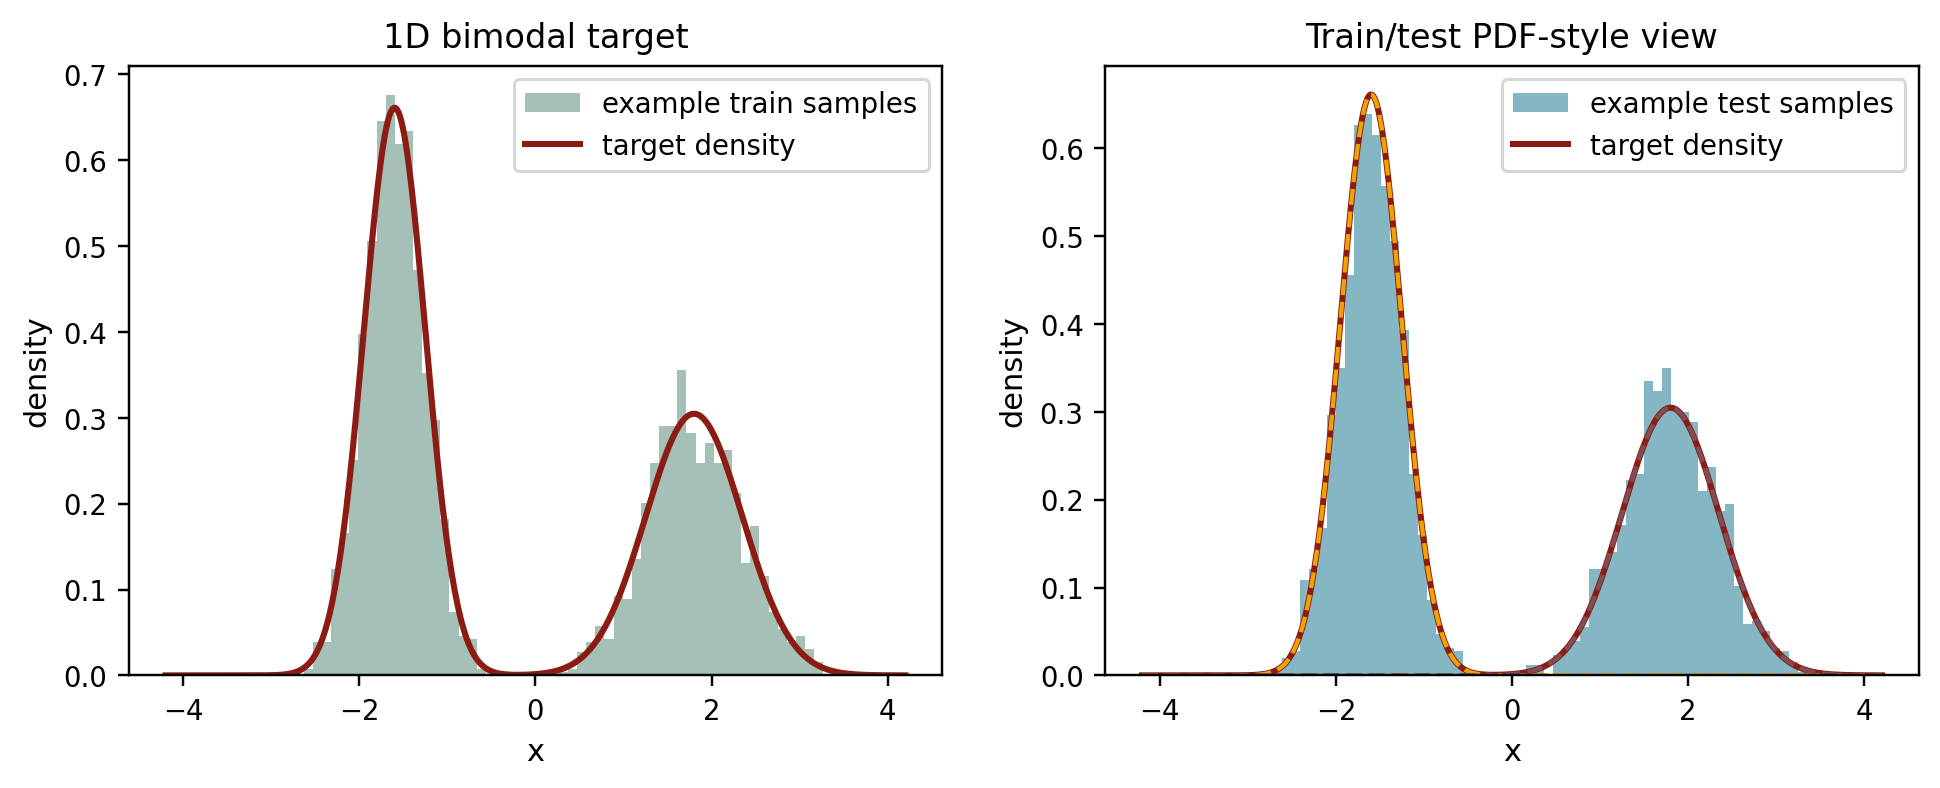
\includegraphics[width=\linewidth]{toy_1d_distribution.png}
    \caption{Exercise 1 target distribution and PDF-style sample comparisons.}
  \end{subfigure}\hfill
  \begin{subfigure}[t]{0.49\linewidth}
    \centering
    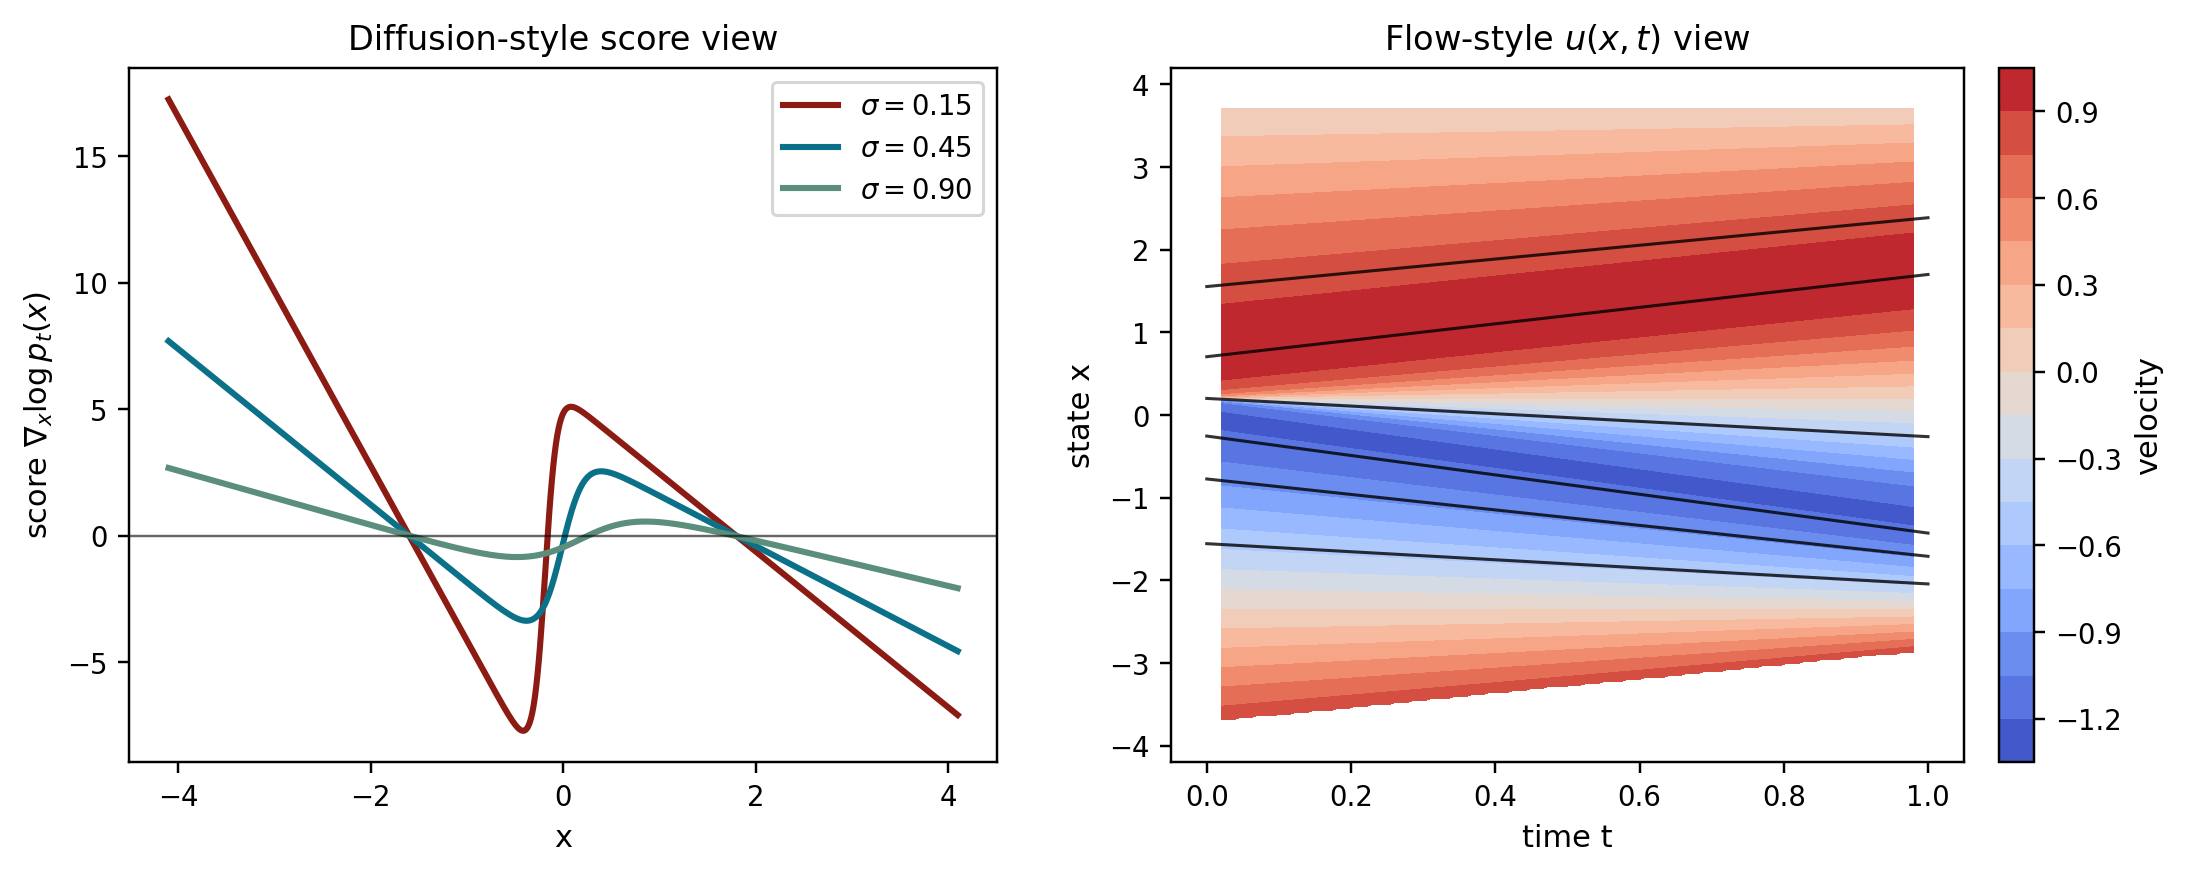
\includegraphics[width=\linewidth]{toy_1d_fields.png}
    \caption{Example method-specific visuals: diffusion score curves and a flow-style $u(x,t)$ view.}
  \end{subfigure}
  \caption{The handout expects both sample comparisons and method-specific geometric views. The panels here are illustrative only. In your report, the corresponding field plots must come from \emph{your trained models}.}
\end{figure}

\section*{Exercise 1: 1D Target Distribution}
Let the data distribution be a bimodal Gaussian mixture
\[
  p_{\mathrm{data}}(x)
  =
  0.58\,\mathcal{N}(x;-1.6,0.35^2)
  +
  0.42\,\mathcal{N}(x;1.8,0.55^2).
\]

\paragraph{Task.}
There is no pre-existing dataset for this problem. First sample your own training, validation, and test sets from this 1D target distribution, then train one diffusion model and one flow-matching model to learn it and generate new samples that match it well.

\paragraph{Questions.}
\begin{enumerate}
  \item Diffusion
  \begin{enumerate}
    \item Build independent training, validation, and test samples from the target distribution. Use the standard diffusion formulation from the lecture:
    \[
      x_t = s_t x_0 + \sigma_t \varepsilon,
      \qquad
      \min_\theta \mathbb{E}\left[\left\lVert \varepsilon_\theta(x_t,t)-\varepsilon \right\rVert^2\right].
    \]
    As a concrete starting point only, you may begin with a fully connected network with 7 hidden layers of width 16, input $(x_t,t)$, scalar output, and \texttt{tanh} activations. This is only an example baseline, not a requirement. Describe the architecture you use.
    \item Train the diffusion model on the training set and generate fresh samples from the trained model.
    \item Compare generated samples against the \textbf{held-out test set} using PDF-style visuals such as histograms or density plots.
    \item Plot training and validation loss curves.
    \item The network predicts $\varepsilon_\theta(x_t,t)$, not the score directly. Using the standard relation implied by the lecture parameterization,
    \[
      \hat{s}_\theta(x_t,t) = -\frac{\varepsilon_\theta(x_t,t)}{\sigma_t},
    \]
    visualize the induced score field estimate for one or more fixed noise levels.
    \item Report the \textbf{1D Wasserstein distance} between generated samples and test samples only.
  \end{enumerate}

  \item Flow Matching
  \begin{enumerate}
    \item Repeat the previous item 1 for flow matching. Use the standard straight-path formulation
    \[
      x_t = (1-t)x_0 + t x_1,
      \qquad
      \min_\theta \mathbb{E}\left[\left\lVert v_\theta(x_t,t) - (x_1-x_0) \right\rVert^2\right].
    \]
    You may reuse the same width-16, 7-layer \texttt{tanh} MLP as an initial example baseline. Again, this is only a starting point, not a requirement.
    \item Repeat the previous item 2 for the trained flow-matching model.
    \item Repeat the previous item 3 for flow matching.
    \item Repeat the previous item 4 for flow matching.
    \item Produce a visualization of the \textbf{trained network's} learned velocity $u_\theta(x,t)$ as a function of both state and time, for example a heatmap or contour plot over $(x,t)$, optionally with representative trajectories overlaid.
    \item Repeat the previous item 6 for flow matching.
  \end{enumerate}
\end{enumerate}

\paragraph{Evaluation note.}
Use a common library implementation of the 1D Wasserstein distance, for example \texttt{scipy.stats.wasserstein\_distance} or the equivalent in your language. Report results on the \textbf{test set only}.

\section*{Exercise 2: 2D Swirl Distribution}
Construct a noisy planar swirl in $\mathbb{R}^2$ by sampling
\[
  \phi \sim \mathrm{Uniform}[1,4\pi],
  \qquad
  \xi_1,\xi_2 \sim \mathcal{N}(0,1),
\]
and then setting
\[
  x =
  \bigl(
    0.18\,\phi\cos\phi + 0.08\,\xi_1,\;
    0.18\,\phi\sin\phi + 0.08\,\xi_2
  \bigr).
\]

\paragraph{Task.}
There is no pre-existing dataset for this problem. First sample your own training, validation, and test sets from this 2D swirl distribution, then train one diffusion model and one flow-matching model to learn it and generate new points on the swirl.

\begin{figure}[t]
  \centering
  \begin{subfigure}[t]{0.49\linewidth}
    \centering
    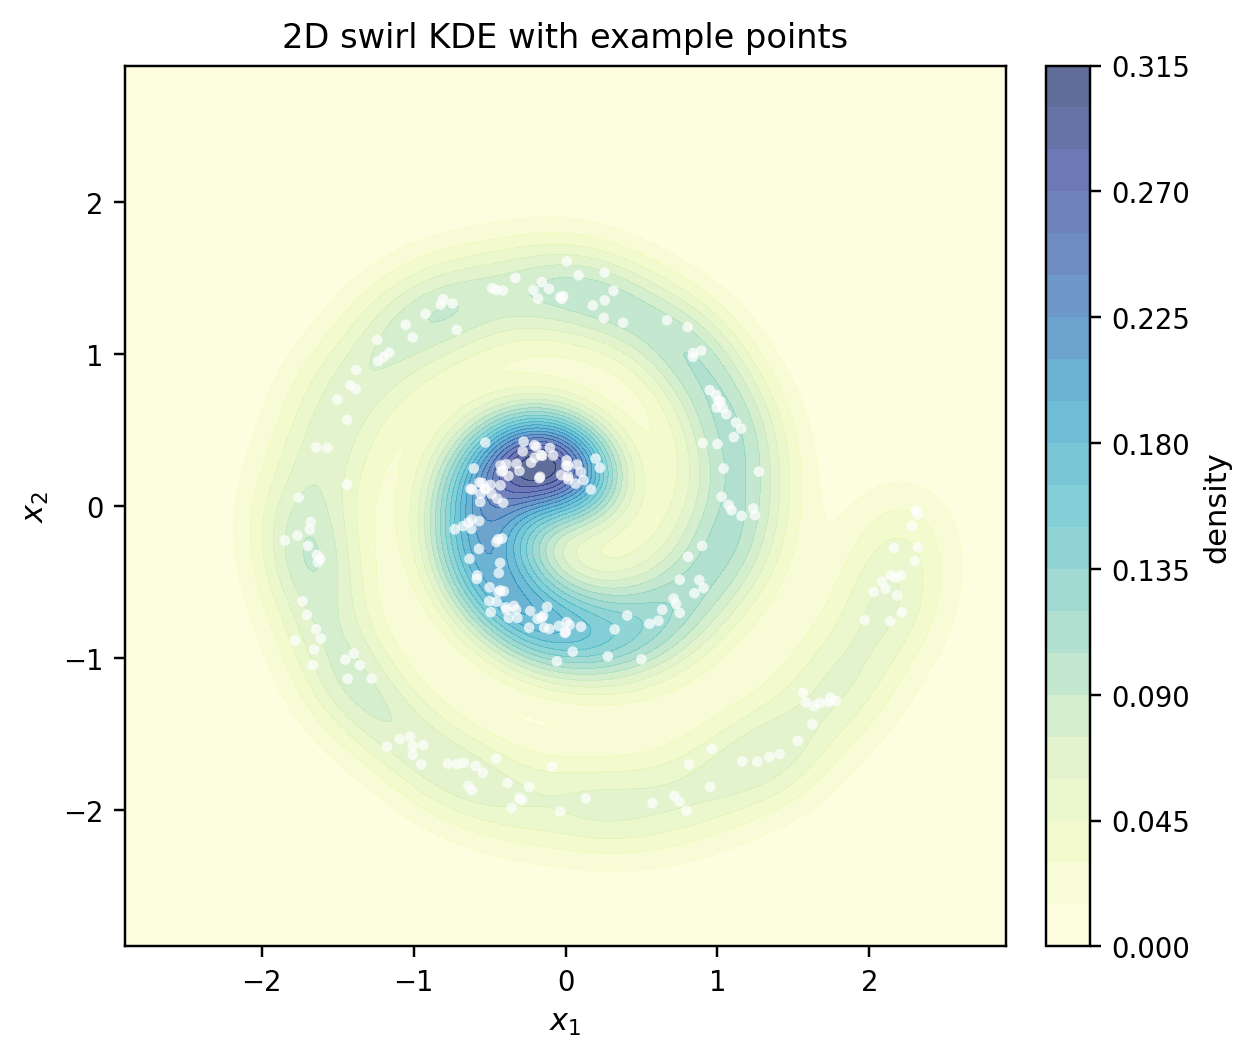
\includegraphics[width=\linewidth]{toy_2d_distribution.png}
    \caption{Exercise 2 target swirl: one KDE axis with example points.}
  \end{subfigure}\hfill
  \begin{subfigure}[t]{0.49\linewidth}
    \centering
    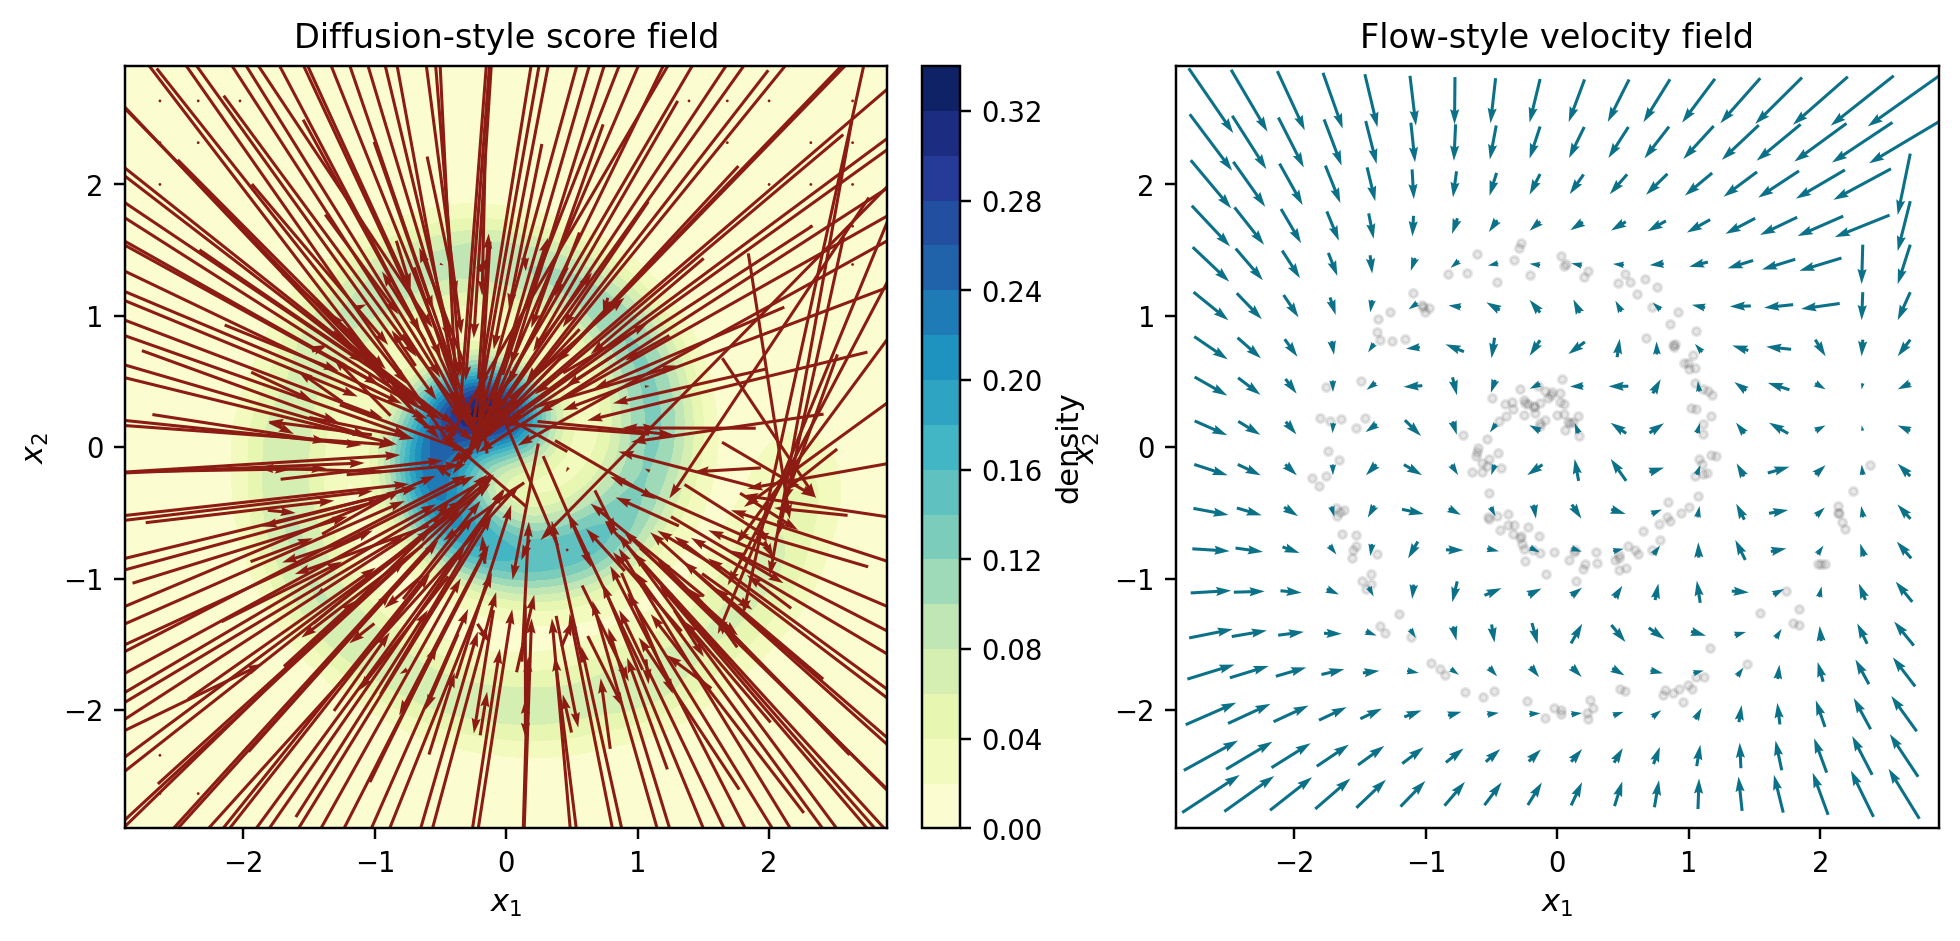
\includegraphics[width=\linewidth]{toy_2d_fields.png}
    \caption{Example method-specific visuals in 2D: score field and flow velocity field.}
  \end{subfigure}
  \caption{For the 2D problem, the report should show both the generated geometry and the learned vector fields behind it. Again, the example panels here are illustrative; your report must visualize the outputs of your trained models.}
\end{figure}

\paragraph{Questions.}
\begin{enumerate}
  \item Diffusion
  \begin{enumerate}
    \item Build independent training, validation, and test samples for the swirl distribution. Use the same standard diffusion formulation as in Exercise 1. As a concrete starting point only, you may begin with a fully connected network with 6 hidden layers of width 12, input $(x_t,t)$ with $x_t \in \mathbb{R}^2$, two outputs, and \texttt{tanh} activations. This is only an example baseline, not a requirement. The repo also includes \texttt{generative/src/solve\_toy\_diffusion\_flow\_2d.py} as a minimal Exercise 2 baseline. Describe the architecture you use.
    \item Train the diffusion model on the training set and generate fresh samples from the trained model.
    \item Compare generated samples against the \textbf{held-out test set} using a scatter plot and a density-style view such as a 2D histogram, KDE, or contour plot.
    \item Plot training and validation loss curves.
    \item Using
    \[
      \hat{s}_\theta(x_t,t) = -\frac{\varepsilon_\theta(x_t,t)}{\sigma_t},
    \]
    produce a quiver plot or similar visualization of the induced score field estimate at one or two fixed noise levels, ideally with sample locations overlaid.
    \item Report an empirical \textbf{2D Wasserstein distance} between generated samples and test samples only, and state exactly which library or function you used.
  \end{enumerate}

  \item Flow Matching
  \begin{enumerate}
    \item Repeat the previous item 1 for flow matching. You may reuse the same width-12, 6-layer \texttt{tanh} MLP as an initial example baseline. Again, this is only a starting point, not a requirement.
    \item Repeat the previous item 2 for the trained flow-matching model.
    \item Repeat the previous item 3 for flow matching.
    \item Repeat the previous item 4 for flow matching.
    \item Produce a vector-field visualization of the \textbf{trained network's} learned velocity $u_\theta(x,t)$ at one representative time, for example with a quiver plot and sample locations overlaid.
    \item Repeat the previous item 6 for flow matching.
  \end{enumerate}
\end{enumerate}

\paragraph{Evaluation note.}
Report results on the \textbf{test set only}.

\section*{General Instructions and Deliverables}
\begin{itemize}
  \item You may use any programming language, framework, or library.
  \item No dataset is provided. In both exercises, you must generate the synthetic data yourself from the distributions in the statement.
  \item Use separate \textbf{training}, \textbf{validation}, and \textbf{test} sets.
  \item All quantitative evaluation must be reported on the \textbf{test set only}.
  \item The deliverable is a concise report of at most \textbf{3--4 pages}.
  \item The report must include:
  \begin{itemize}
    \item a brief statement of each problem,
    \item the chosen architecture and why it is appropriate,
    \item the training procedure and important hyperparameters,
    \item train and validation loss curves,
    \item the required sample visualizations,
    \item the diffusion score-field visualizations computed from $\hat{s}_\theta(x_t,t) = -\varepsilon_\theta(x_t,t)/\sigma_t$,
    \item the flow-matching velocity-field visualizations,
    \item the \textbf{test-set-only} Wasserstein results,
    \item a short comparison between diffusion and flow matching.
  \end{itemize}
\end{itemize}

\vspace{0.75em}
\noindent\textbf{References.}
Ho et al., \emph{Denoising Diffusion Probabilistic Models}, NeurIPS 2020. \\
Lipman et al., \emph{Flow Matching for Generative Modeling}, ICLR 2023. \\
SciPy Wasserstein distance documentation:
\url{https://docs.scipy.org/doc/scipy/reference/generated/scipy.stats.wasserstein_distance.html}

\end{document}
